%!TEX root = ../thesis.tex
%*******************************************************************************
%****************************** Third Chapter **********************************
%*******************************************************************************
\chapter{The electron-removal method for boosted \teth reconstruction}

\graphicspath{{1_MainChapters/Chap6_ElecRM/figs/}}

\section{Introduction}
    \label{sec:erm:intro}
    Similar to the \tmth channel, if an electron lies within the \tauseed jet,
    the standard TauReco and TauID algorithm is not able to reconstruct and identify the \tauhad. 
    Figure \ref{fig:erm:dR_eff_off} shows the combined reconstruction and 
    identification efficiency as a function of the truth-level $\dRvistt$. 
    The efficiency of the TauReco and TauID algorithms drop significantly when the $\dRvistt$ is less than 0.4, as the electron begin to merge with the \tauseed jet. As a result, the 
    possibility of reconstructing the correct number of \tauhad tracks is significantly reduced, 
    and the \tauhad identification efficiency drops significantly in all the WPs.
    \begin{figure}[htbp]
        \centering
        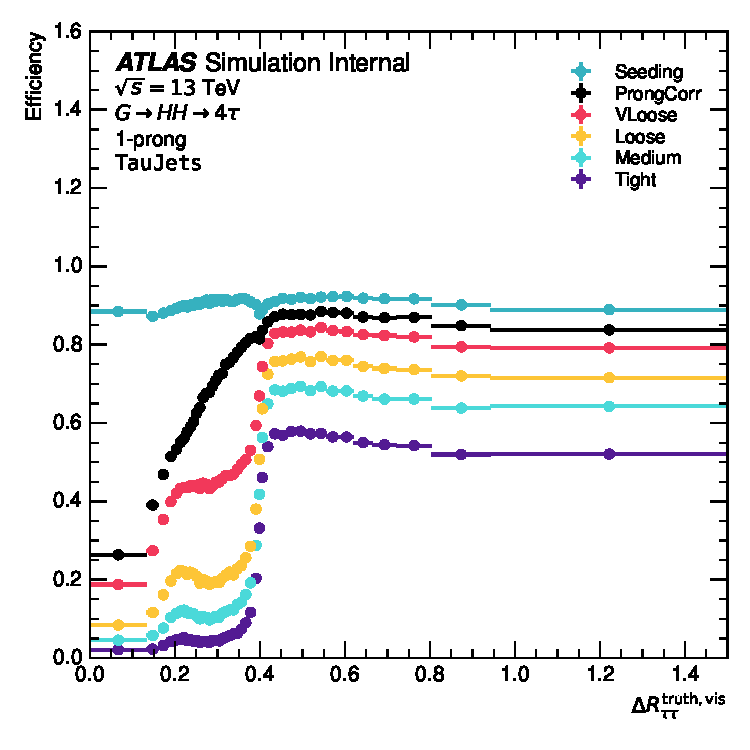
\includegraphics[width=0.495\textwidth]{plots_dev/eff_nocut_dR_off_1p.pdf}
        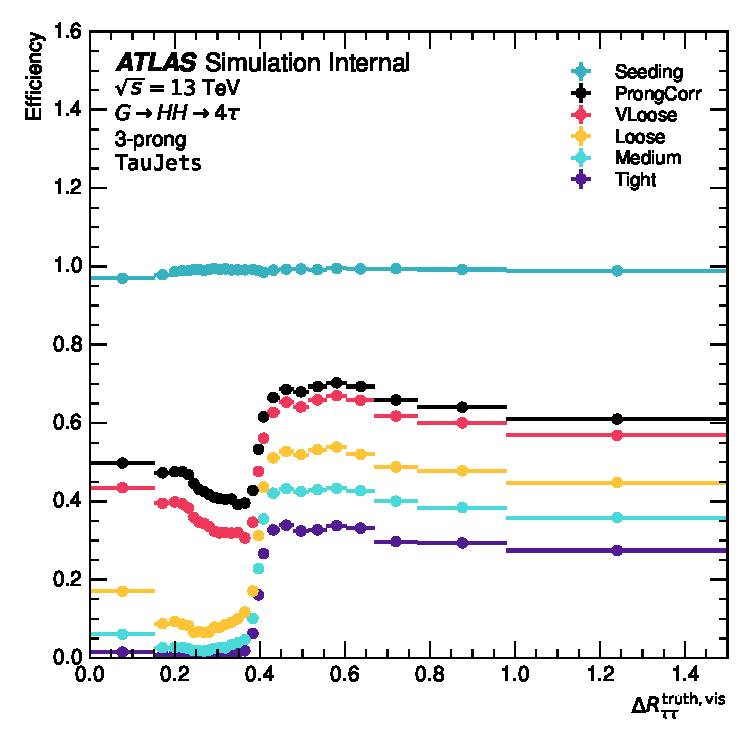
\includegraphics[width=0.495\textwidth]{plots_dev/eff_nocut_dR_off_3p.pdf}
        \caption{The combined reconstruction and identification efficiency of the 
        standard TauReco and TauID as a function of the truth-level $\dRvistt$. The
        efficiency is shown for the different working points of the TauID algorithm. 
        In addition, the ``Reco'' and ``ProngCorr'' efficiencies are shown, 
        which are the efficiency of the \tauhad being seeded, and the efficiency 
        of the TauRec algorithm to reconstruct the correct number of tracks in the 
        \tauhad, respectively.}
        \label{fig:erm:dR_eff_off}
    \end{figure}
    Having demonstrated the success of the \tauhadmurm, we proposed a 
    similar method for the \teth channel, the electron-removal \tauhad (\tauhaderm).

    The \tauhaderm reconstruction is however much more challenging 
    than the \tauhadmurm, technically and physically.
    The electron is not a minimum ionising particle (MIP) like the muon.
    Its energy deposition in the calorimeter makes it much more complicated to remove.
    The electron showers in the calorimeter, depositing most of its energy 
    in the EM calorimeter. In very highly boosted cases, 
    the electron can also deposit significant energy in the hadronic calorimeter. 
    In the context of the \tauhaderm, the electron cluster can merge with 
    the \tauhad clusters, making the separation of the clusters difficult.
    The presence of the electron in the \tauseed jet can also drag the barycentre 
    of the \tauhad to the direction of the electron. 
    Simply removing the electron from the \tauseed jet results in a \tauhad with 
    a shifted axis. with some of the \tauhad decay products being outside 
    the core-cone of the \tauseed jet. This problem severely affects the efficacy of a
    simple electron-removal method. 

    In Section~\ref{sec:erm:method}, we present an accretive method to reconstruct the 
    \tauhaderm in the presence of an electron. We also show that the accretive 
    \tauhaderm can be reconstructed with high 
    efficiency in the region where the $\dRvistt > 0.2$. 
    The energy and spatial resolution of the \tauhaderm are presented in
    Section~\ref{sec:erm:ereso}.
    An initial benchmark of the \tauhaderm in the \Zttehad channel is presented 
    in Section~\ref{sec:erm:benchmark}.
    The summary and outlook of the \tauhaderm reconstruction is presented 
    in Section~\ref{sec:erm:summary}.

\section{Accretive $\tauhaderm$ reconstruction method}
    \label{sec:erm:method}
    For the development of \tauhaderm, the \GHHFourtau MC samples as described in Chapter 5 are used. 
    However, instead of utilising the full mass range of the \GHHFourtau 
    samples, only the $m_G=1500$ \GeV sample is considered due to limitations in resources for 
    custom ATLAS MC production.
    This sample is chosen because it covers the $\Delta R^\mathrm{truth}_\mathrm{\tau\tau}$ 
    range from 0.1 to 0.6, which represents the most comprehensive region for \tauhaderm reconstruction.
    The accretive \tauhaderm reconstruction is a six-step process for every event:
    \begin{enumerate}
        \item The first step is to identify the electrons that satisfy the MediumLH WP, without isolation requirements.
        \item The second step is to remove the tracks and calorimeter clusters associated with the electrons from the event.
        \item Thirdly, using the remaining LCTopo clusters and tracks, the \tauseed jets are re-clustered with the \antikt algorithm with $R=0.4$.
        \item In the fourth step, re-clustered electron-free \tauseed jets with $\dRttReco > 0.6$ to any identified electron are removed from the event, as they should not be affected by the electron.
        \item Then, the electron-free track and cluster collections are supplied to the TauRec algorithm, which reconstructs the \tauhaderm candidates from the remaining \tauseed jets.
        \item Finally, the \tauhaderm candidates are identified using the standard TauID algorithm.
    \end{enumerate}

    Figure \ref{fig:erm:eff_dR_erm} shows the TauID efficiency of the accretive \tauhaderm reconstruction method as a function of the truth-level $\dRvistt$.
    \begin{figure}[htbp]
        \centering
        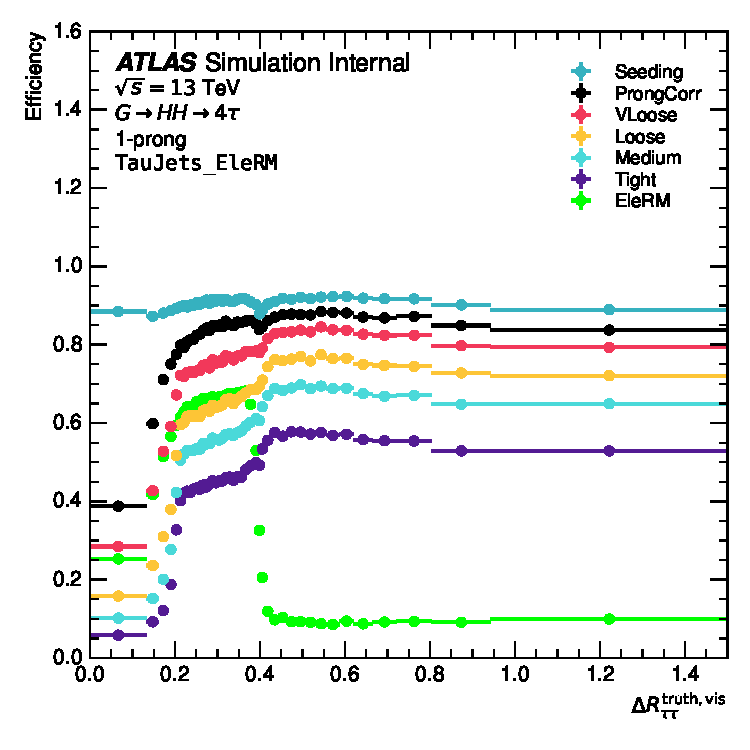
\includegraphics[width=0.495\textwidth]{plots_dev/eff_nocut_dR_new_1p.pdf}
        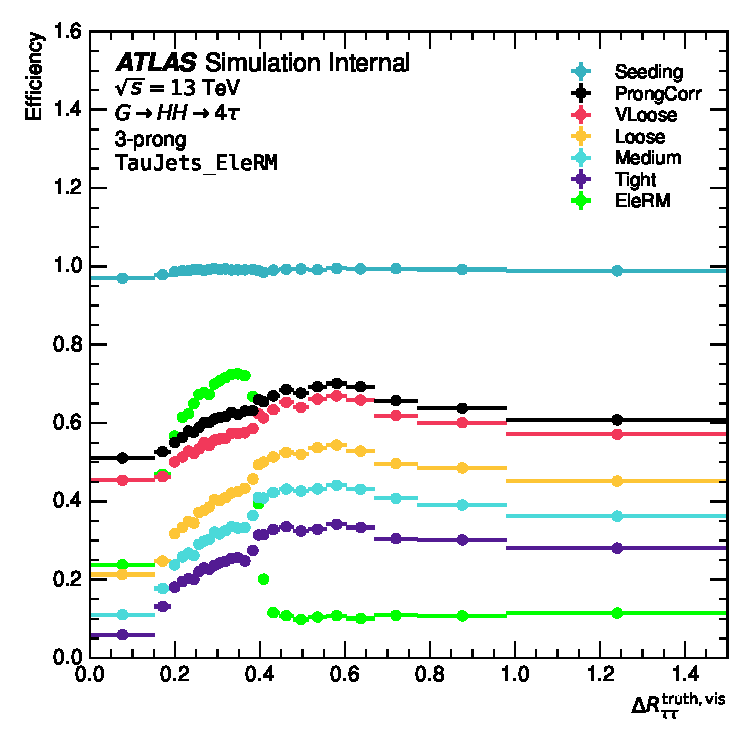
\includegraphics[width=0.495\textwidth]{plots_dev/eff_nocut_dR_new_3p.pdf}
        \caption{The combined reconstruction and identification efficiency of the accretive \tauhaderm reconstruction method as a function of the truth $\dRvistt$. The
        efficiency is shown for every working points of the TauID algorithm. In addition, the ``Reco'', ``ElecRM'', and ``ProngCorr'' efficiencies are shown, which is the efficiency of the
        \tauhad being seeded, the efficiency of the electron-removal, and the efficiency of the TauRec algorithm reconstructing the correct number of tracks, respectively.}
        \label{fig:erm:eff_dR_erm}
    \end{figure}
    Compared to more than 90\% MediumLH efficiency for isolated electrons at high \pT~\cite{EGAM-2021-01}, 
    the ``ElecRM'' efficiency is significantly lower, at around 70\% in $\dRvistt > 0.2$ region. 
    Below this threshold, the electron ID efficiency drops significantly, as the electron and \tauhad clusters start to merge. 
    The TauID efficiency of the \tauhaderm is significantly 
    higher than the standard TauID algorithm in this region,
    but not as high as the TauID efficiency for isolated \tauhad candidates.

    If we only consider the case where the overlapping electron is identified and removed, the performance as functions of truth-level 
    $\dRvistt$, $\pT{}_{\tau}^\mathrm{truth,vis}$, and $|\eta|^\mathrm{truth, vis}$ are shown in 
    Figure \ref{fig:erm:eff_new_trkrm}.
    In such cases, the TauID efficiency in various WPs in the $\dRvistt > 0.2$ 
    region are completely recovered.
    The ``ProngCorr'' efficiency is also recovered to more than 90\% in the $\dRvistt > 0.2$ 
    region for 1-prong \tauhaderm.
    The ``ProngCorr'' efficiency reaches 80\% for 3-prong \tauhaderm at low-\pT. 
    In 3-prong case, higher track multiplicity makes it more challenging to reconstruct \tauhad, especially in high \pT region.
    When the electron is identified and removed, the TauID efficiency
    behaves similarly to the standard TauID algorithm and the muon-removal method. 
    The similarity shows that the accretive \tauhaderm 
    objects can be treated as isolated \tauhad objects.
    In all cases, the electron-removal, TauRec, and TauID efficiencies drops significantly in 
    the $\dRvistt < 0.2$ region. As the electron and \tauhad clusters start to merge in this region, 
    both the identification of the electron and the reconstruction of the \tauhad becomes more challenging.

    \begin{figure}[htbp]
        \centering
        \subfloat[]{
            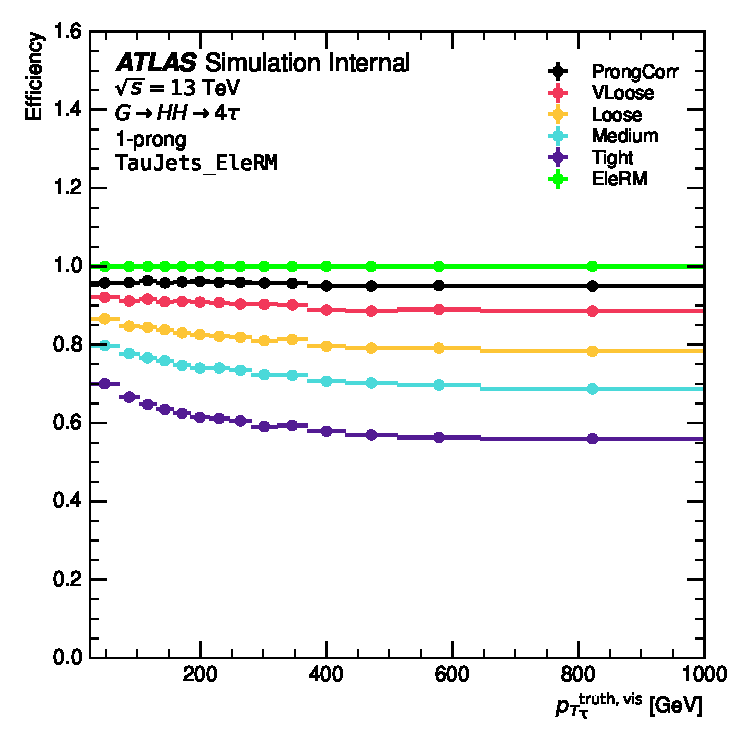
\includegraphics[width=0.5\textwidth]{plots_dev/eff_02dR04_erm_pt_new_1p.pdf}
            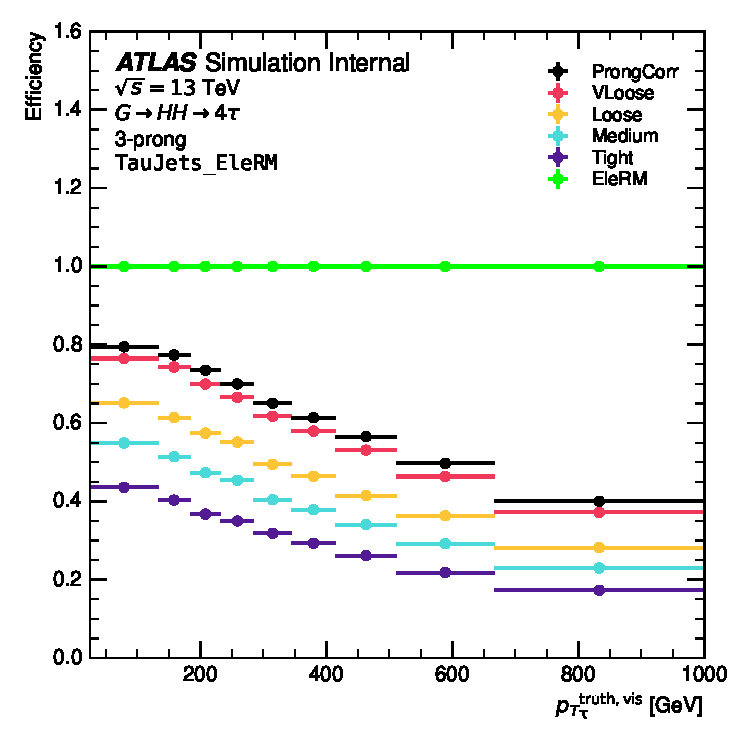
\includegraphics[width=0.5\textwidth]{plots_dev/eff_02dR04_erm_pt_new_3p.pdf}
            \label{fig:eff_pt_new_trkrm_unique}
        }
        \\
        \subfloat[]{
            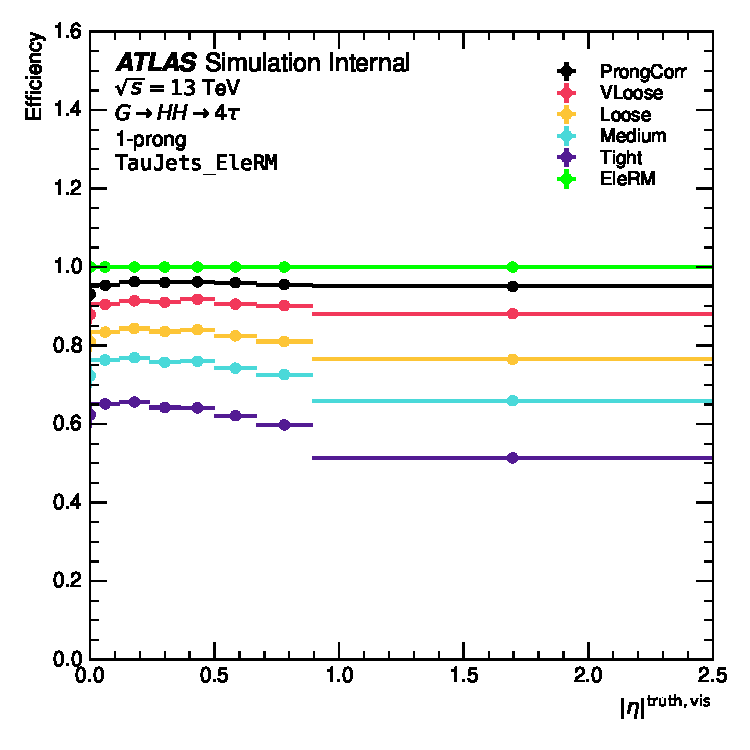
\includegraphics[width=0.5\textwidth]{plots_dev/eff_02dR04_erm_eta_new_1p.pdf}
            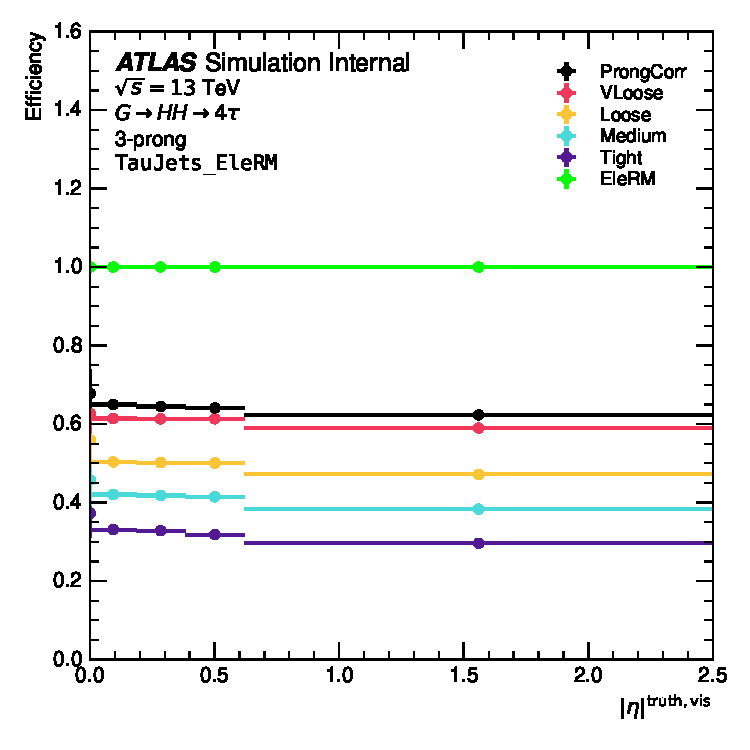
\includegraphics[width=0.5\textwidth]{plots_dev/eff_02dR04_erm_eta_new_3p.pdf}
            \label{fig:eff_abseta_new_trkrm}
        }
        \caption{The efficiency of the accretive \tauhaderm reconstruction method as a function of the truth-level
        $\pT{}_{\tau}^\mathrm{truth,vis}$ (\protect\subref{fig:eff_pt_new_trkrm_unique}), 
        and $|\eta|^\mathrm{truth, vis}$ (\protect\subref{fig:eff_abseta_new_trkrm}), 
        where the electron is identified and removed. The
        efficiency is shown for the different working points of the TauID algorithm for 1-prong and 3-prong. In addition, the ``ElecRM'', and ``ProngCorr'' efficiencies are 
        the efficiency of the electron-removal, and 
        the efficiency of the TauRec algorithm to reconstruct the correct number of tracks in the \tauhad, respectively.}
        \label{fig:erm:eff_new_trkrm}
    \end{figure}

    This method is much more challenging technically compared to the case for \tauhadmurm, 
    due to the limitations of the event-level thinning in the ATLAS xAOD Event Data Model (EDM). 
    TauRec algorithms rely on the individual calorimeter cell information to function.
    After the ATLAS Tier-0 reconstruction, the calorimeter cell information is discarded 
    unless they are associated with a reconstructed standard \tauhad candidates.
    The \tauhaderm objects contains different clusters than the standard \tauhad objects, 
    in which the cells are not preserved in the xAOD.
    As a result, the \tauhaderm reconstruction is not possible in the standard ATLAS xAOD EDM. 
    It can only be performed in the ATLAS Tier-0 reconstruction. 
    The \tauhaderm objects originate from a different set of $\tauseed$ jets,
    meaning that unlike the $\tauhadmurm$, there is no direct equivalent in the standard \tauhad collection. 
    To save Tier-0 CPU usage and xAOD storage, only the \tauhaderm objects that are within 
    $\dRvistt < 0.6$ are saved in the xAOD.

\section{Energy and spatial resolution of the \tauhaderm}
    \label{sec:erm:ereso}
    \begin{figure}[!tb]
        \centering
        \subfloat[]{
            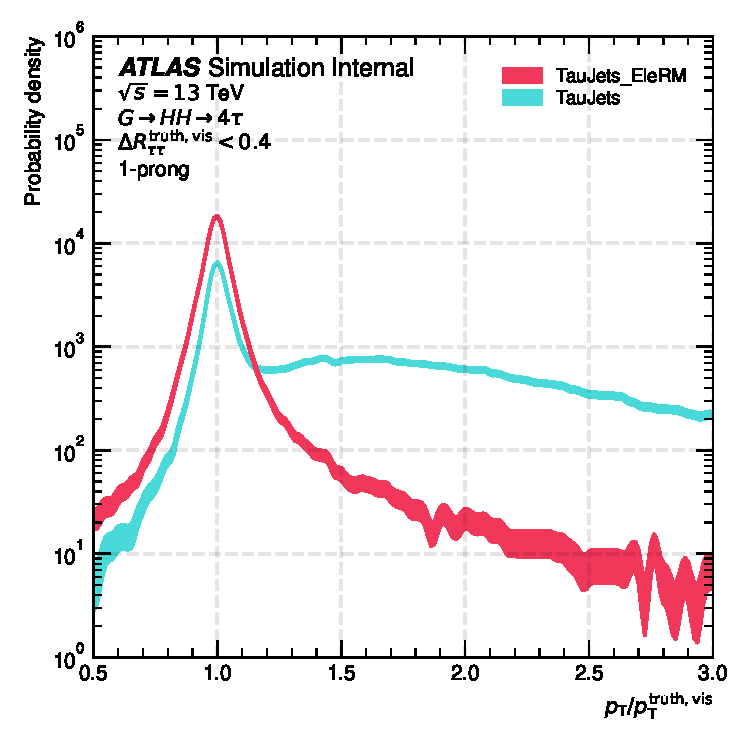
\includegraphics[width=0.5\textwidth]{plots_dev/reso_pt_diff_1p.pdf}
            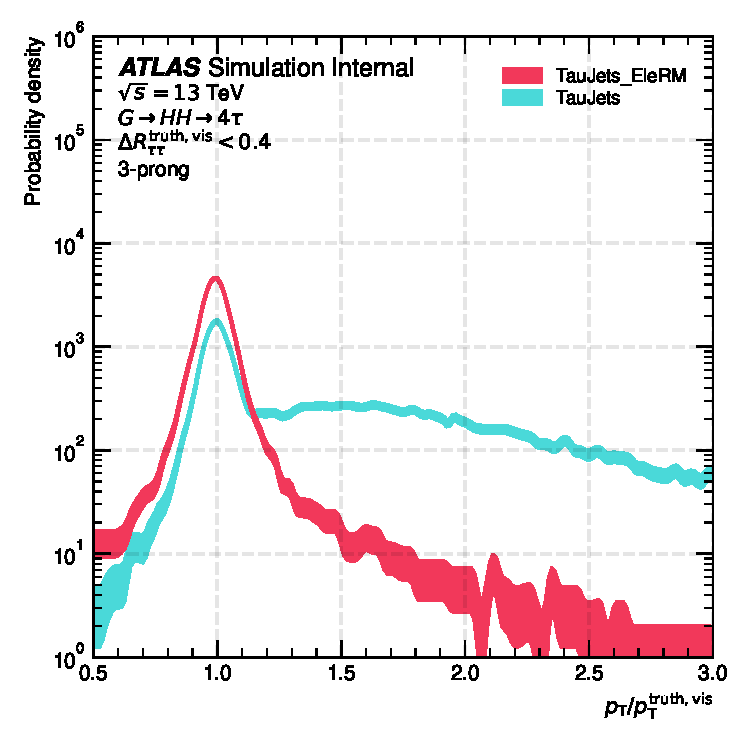
\includegraphics[width=0.5\textwidth]{plots_dev/reso_pt_diff_3p.pdf}
            \label{fig:diff_pt}
        }
        \\
        \subfloat[]{
            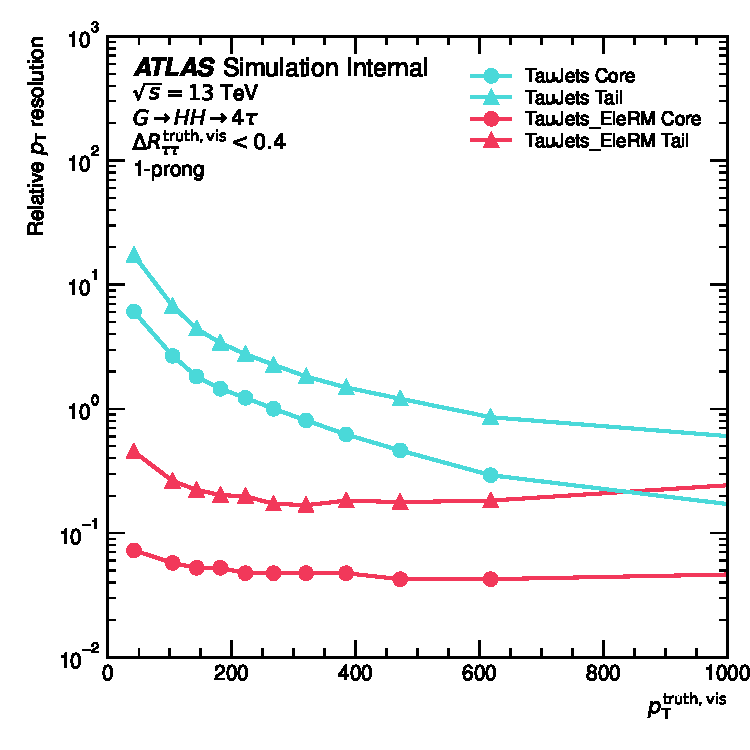
\includegraphics[width=0.5\textwidth]{plots_dev/reso_rela_pt_1p.pdf}
            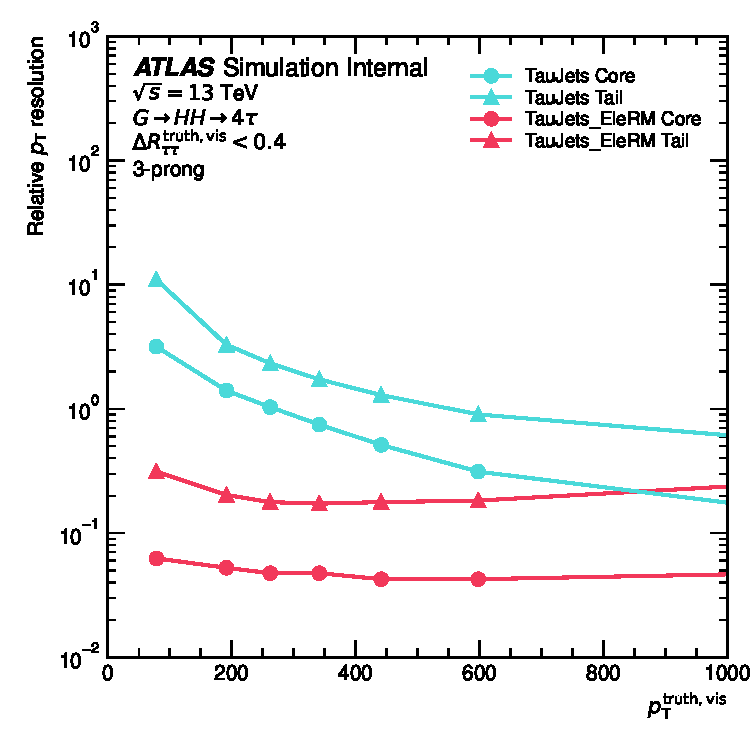
\includegraphics[width=0.5\textwidth]{plots_dev/reso_rela_pt_3p.pdf}
            \label{fig:ereso_abseta_new_trkrm}
        }
        \caption{The distributions of the calibrated transverse energy residuals for $\tauhadvis$ with
                \tauhaderm (red) and \tauhad (blue) are shown in (\protect\subref{fig:diff_pt}). 
                The relative core (68\%) and tail (95\%) $\tauhadvis$ $p_\mathrm{T}$ resolutions as functions of
                $\pT{}_{\tau}^\mathrm{truth,vis}$ are shown in  (\protect\subref{fig:ereso_abseta_new_trkrm}). 
                The left plots show the 1-prong case and the right plots show the 3-prong case.}
        \label{fig:erm:ereso_trkrm}
    \end{figure}
    Having demonstrated the TauID efficiency of the \tauhaderm, we now turn our 
    attention to the energy and spatial resolution of the \tauhaderm.
    The relative energy resolution ($\frac{p^\mathrm{reco}_\mathrm{T}}{p^\mathrm{truth}_\mathrm{T}}$) 
    of the \tauhaderm is shown in Figure \ref{fig:erm:ereso_trkrm}.
    The spatial resolution of the \tauhaderm in terms of the difference in the 
    truth and reconstructed $\phi$ and $\eta$ are shown in Figure \ref{fig:erm:spatialreso_trkrm}. 
    \begin{figure}[!tb]
        \centering
        \subfloat[]{
            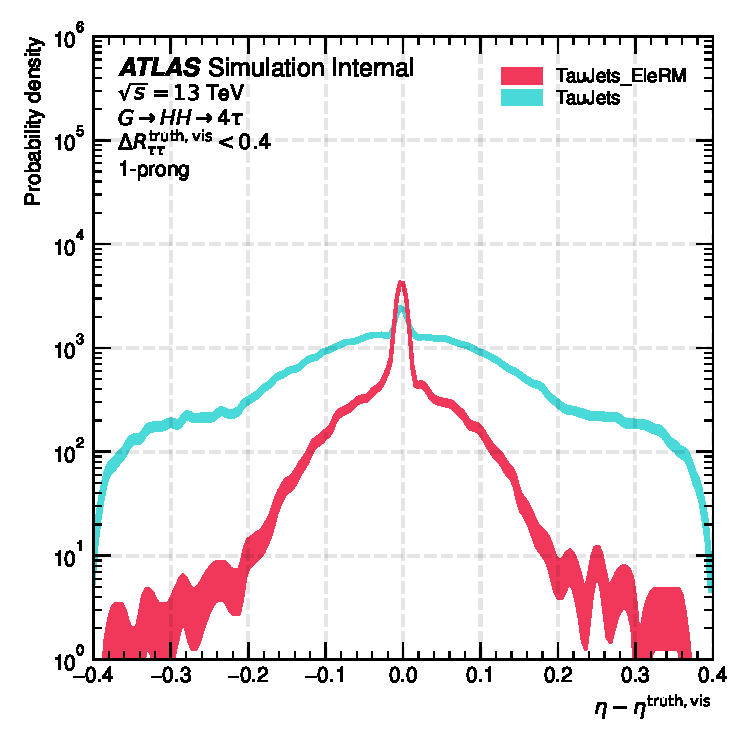
\includegraphics[width=0.5\textwidth]{plots_dev/reso_eta_diff_zoom_1p.pdf}
            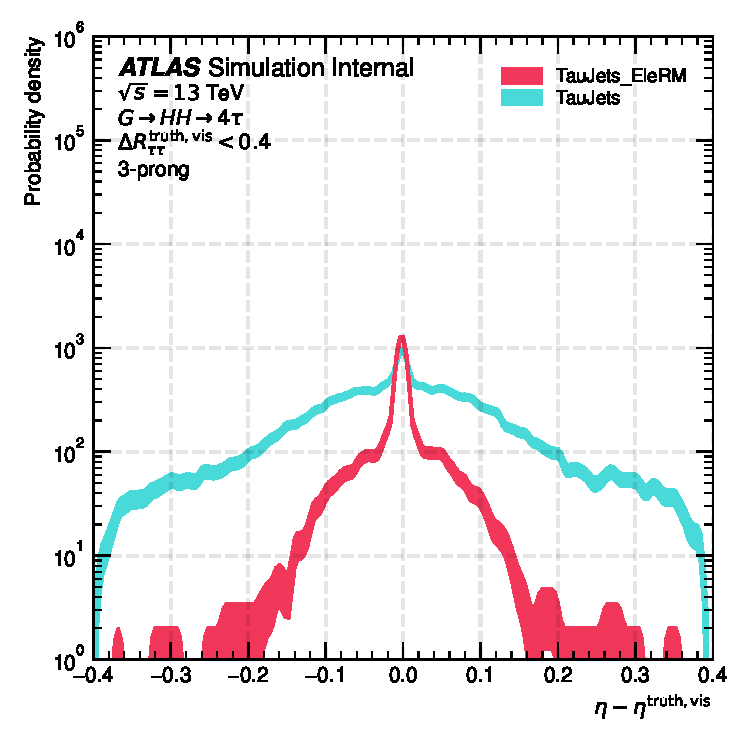
\includegraphics[width=0.5\textwidth]{plots_dev/reso_eta_diff_zoom_3p.pdf}
            \label{fig:dphi_reso}
        }
        \\
        \subfloat[]{
            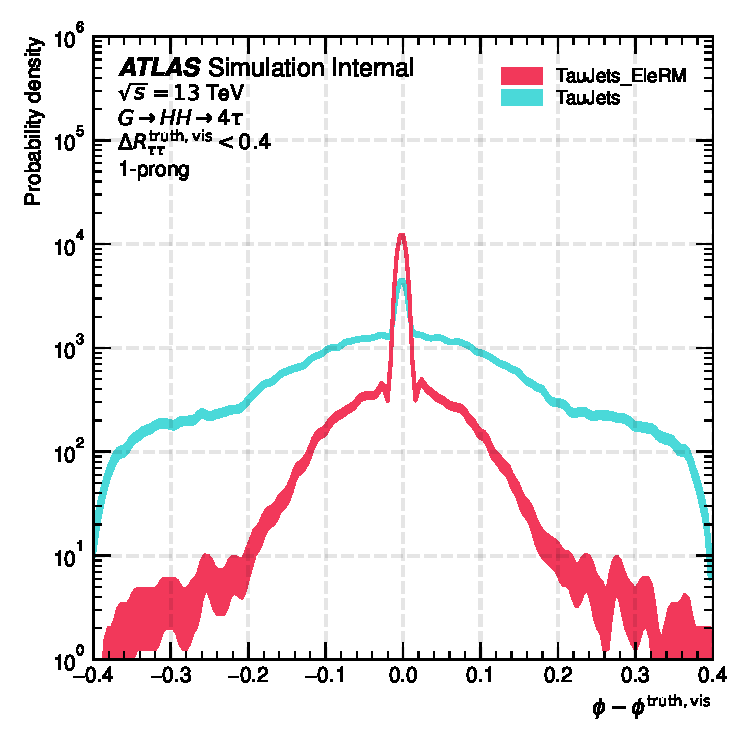
\includegraphics[width=0.5\textwidth]{plots_dev/reso_phi_diff_zoom_1p.pdf}
            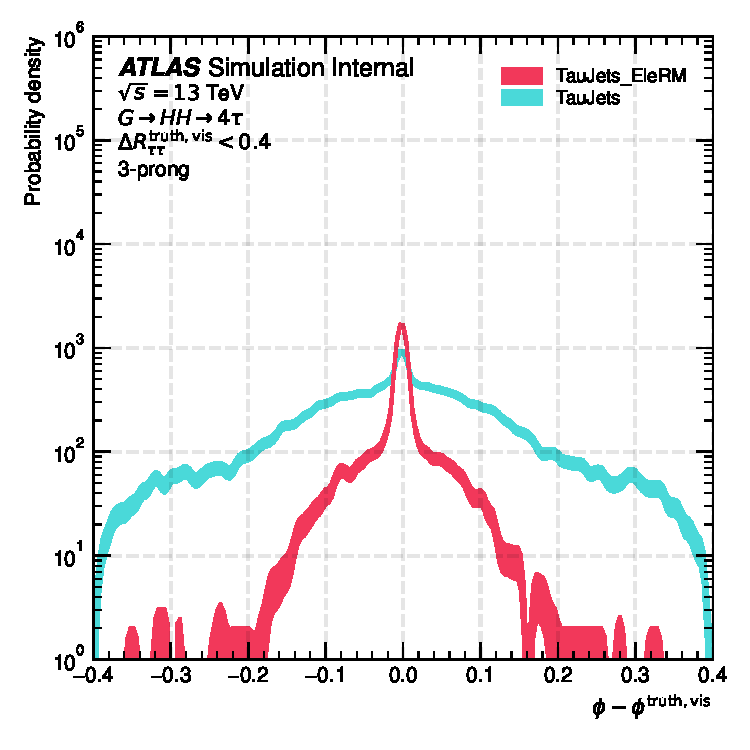
\includegraphics[width=0.5\textwidth]{plots_dev/reso_phi_diff_zoom_3p.pdf}
            \label{fig:deta_reso}
        }
        \caption{The distributions of the $\phi$ (\protect\subref{fig:dphi_reso}) 
            and $\eta$ (\protect\subref{fig:deta_reso}) residuals for $\tauhadvis$ with
            \tauhaderm (red) and \tauhad (blue) are shown. The left plots show the 1-prong 
            case and the right plots show the 3-prong case.}
        \label{fig:erm:spatialreso_trkrm}
    \end{figure}
    The \tauhaderm objects show significantly
    better energy and spatial resolution than the standard \tauhad objects. 
    Before the electron-removal, the \tauhad objects have a significant upper tail in the energy resolution,
    from the electron calorimeter deposit. The energy resolution of \tauhaderm objects is much improved. 
    Order-of-magnitude improvements are observed in both 1- and 3-prong cases in energy residuals. 
    For the spatial resolution, without the electron dragging on the \tauseed jet barycentre, the \tauhaderm 
    objects have a order-of-magnitude smaller $\phi$ and $\eta$ tails and significantly higher peaks, 
    compared to the standard \tauhad objects. 
    

\section{Benchmark of the \tauhaderm in the \Zttehad channel}
    \label{sec:erm:benchmark}
    Since the reconstruction of \tauhaderm objects runs on the ATLAS Tier-0 reconstruction, they
    have only become available in the ATLAS 2024 data collection. 
    Thanks to the exceptional 2024 operation of  
    LHC and ATLAS, at the time of writing, ATLAS has collected a large amount of data in 2024 that 
    corresponds to an integrated luminosity of 91~\ifb. 
    For now, the benchmark of the \tauhaderm in the \Zttehad channel is performed with the data currently available. 
    Not all the data collected is suitable for physics analysis, but the "Good Run List" (GRL)~\cite{DAPR-2018-01} 
    is not available at the time of writing. 
    From the previous Run-3 operations~\cite{ATL-DAPR-PUB-2023-001}, we estimate that
    around 85 \ifb of the data collected is suitable for physics analysis.
    A complete Run-3 reprocessing of the 2022-2023 data is scheduled for the fourth-quarter of 2024, 
    which will include the reconstruction of \tauhaderm objects.
    At the end of 2024, we will have the \tauhaderm objects in the full Run-3 data, 
    corresponding to a projected integrated luminosity of around 160~\ifb.

    The \tauhaderm has been scheduled for the ATLAS MC samples for 2024 data-taking conditions.
    Unfortunately, at the time of writing, no MC sample that contain \tauhaderm is available due
    to previously unforeseen delays in the MC validation and production. 
    In the coming years, MC samples for the 2022 and 2023 data-taking conditions will be reprocessed with 
    the \tauhaderm objects included.

    \subsection{Event-selection}
        \begin{table}[!hbtp]
            \caption{Summary of event-selection requirements for the \Zttehad channel.}
            \label{tab:erm:evtsel_unique}
            \centering
            % \scriptsize
            \begin{tabular}{lc}
                \toprule
                Object          & Selection \\
                \midrule
                Triggers        & \begin{tabular}{c} 
                                    \texttt{HLT\_xe65\_cell\_xe90\_pfopufit\_L1XE50} \\ 
                                    \texttt{HLT\_e26\_lhtight\_ivarloose\_L1eEM26M} \\ 
                                    \texttt{HLT\_e60\_lhmedium\_L1eEM26M} \\ 
                                    \texttt{HLT\_e140\_lhloose\_L1eEM26M} 
                                \end{tabular} \\
                \midrule
                $\tauhaderm$    & \begin{tabular}{c} 
                                    $0 < |\eta| < 1.37$ or $1.52 < |\eta| < 2.5$ \\ 
                                    Jet RNN score > 0.15 \\
                                    e-veto RNN score > 0.05 \\
                                    $\pt > 15~\GeV$ \\
                                \end{tabular} \\
                \midrule
                $e$             & \begin{tabular}{c} 
                                    $\pt > 10~\GeV$ \\ 
                                    ``MediumLH'' ID \end{tabular} \\
                \midrule    
                $\teth$ system & \begin{tabular}{c} 
                                    $\Delta R(e,\tauhaderm) < 0.4$ \\
                                    $-0.1 < \deltaemet < 0.4$ \\
                                    $\mcolEtau > 40~\GeV$ \\ 
                                    $\ptcolEtau > 250~\GeV$ \\ 
                                    no b-tag jet at 85\% efficiency working point 
                                \end{tabular} \\
                \bottomrule
            \end{tabular}
        \end{table}
        The event-selection and the \teth collinear reconstruction in the \Zttehad channel is very similar to 
        the \tauhadmurm benchmark, with the \tauhadmurm replaced by the \tauhaderm. 
        Exceptions include the trigger requirements, the slightly tighter jet RNN score requirements, 
        and a loose electron-veto RNN requirement.
        event-selection requirements in the \Zttehad channel are summarised in Table~\ref{tab:erm:evtsel_unique}. 
        In addition to these selections, the \tauhaderm in the SR are required to have 
        opposite charge to the electron. 
        The \tauhaderm in the CR is required to have same charge to the electron. 
        The fraction of the selected events that pass the specified triggers is 80\%. 
        The actual trigger efficiency is by definition lower than this value, 
        which is significantly lower than the 97\% observed in the \tmth benchmark SR.
        The \MET trigger efficiency is considerably lower compared to the $\Zttmuhad$
        benchmark, which is expected due to the calorimeter deposit from the electron.
        
    \subsection{Results}
    Without MC samples, the exact composition of the events in the analysis regions is not known. 
    Instead, we rely on kinematic distributions, TauID distributions, and event yields in the SR and CR
    to understand the background level and signal purity in the \Zttehad channel. 
    From the \tauhadmurm benchmark, we know that the highly boosted \Zttmuhad channel is very clean, 
    with a high purity of \tmth events and minimal background. 
    We shall demonstrate below that the \tauhaderm benchmark in the 
    \Zttehad channel is expected to show similar traits in the highly
    boosted \Zttehad channel, given the similar characteristics found during the
    \tauhaderm and \tauhadmurm developments.

    The \teth collinear mass (\mcolEtau), transverse momentum (\ptcolEtau), the \tauhaderm TauID RNN score, 
    and TauID eveto score distributions are shown in Figure \ref{fig:erm:m_col}-\ref{fig:erm:eveto_rnn}, respectively. 
    The SR distributions provide an estimation of the combined signal and background level, 
    whereas the CR distributions give an estimation of the background level.
        \begin{figure}[!tb]
            \centering
            \subfloat[]{
                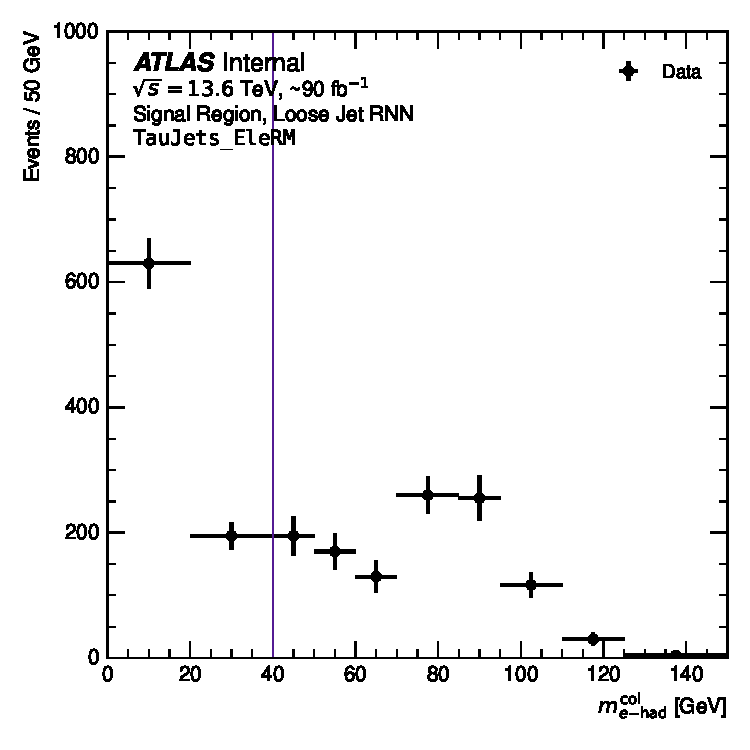
\includegraphics[width=0.50\textwidth]{plotsZtt/erm/erm_m_tt_colin_SR.pdf}
                \label{fig:SR_m_col}
            }
            \subfloat[]{
                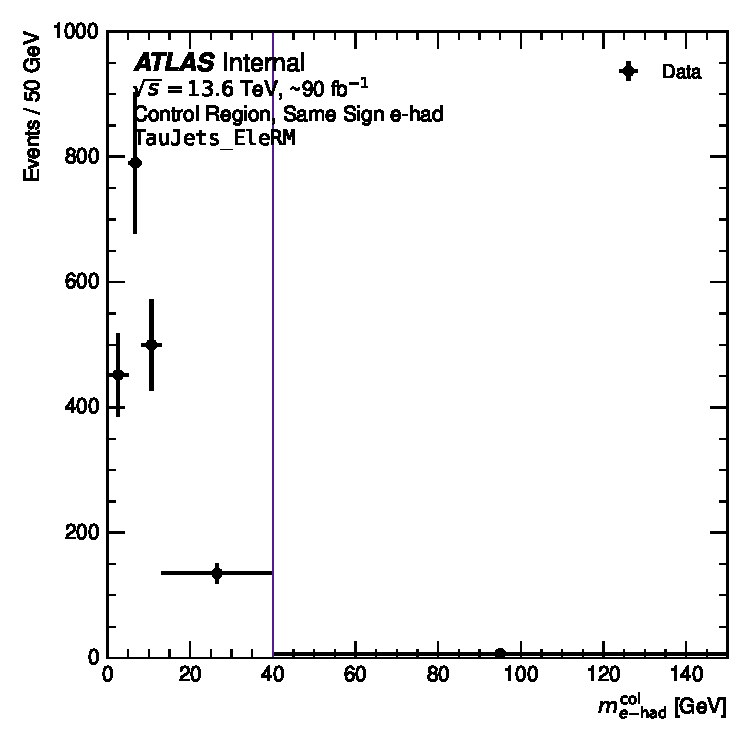
\includegraphics[width=0.50\textwidth]{plotsZtt/erm/erm_m_tt_colin_CR_SS.pdf}
                \label{fig:CR_m_col}
            }
            \caption{
                The distribution of the $\mcolEtau$: (\protect\subref{fig:SR_m_col}) in the SR, and,
                (\protect\subref{fig:CR_m_col}) in the CR. 
                All requirement criteria are applied, 
                except the requirement on the variable being plotted.
                The vertical line indicates the event-selection requirement on this variable.
            }
            \label{fig:erm:m_col}
        \end{figure}
        \begin{figure}[!tb]
            \centering
            \subfloat[]{
                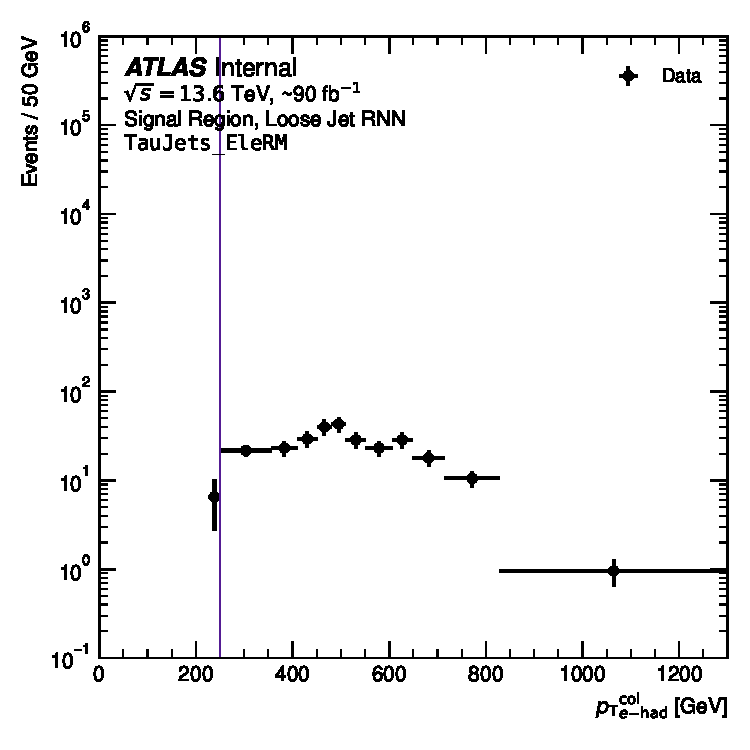
\includegraphics[width=0.50\textwidth]{plotsZtt/erm/erm_pt_tt_colin_SR.pdf}
                \label{fig:SR_pt_col}
            }
            \subfloat[]{
                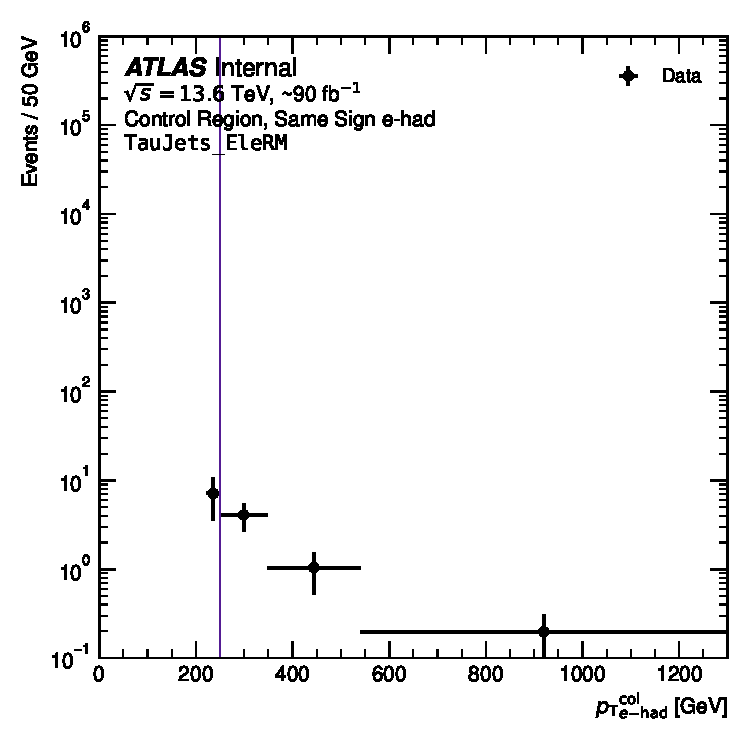
\includegraphics[width=0.50\textwidth]{plotsZtt/erm/erm_pt_tt_colin_CR_SS.pdf}
                \label{fig:CR_pt_col}
            }
            \caption{
                The distribution of the $\ptcolEtau$: (\protect\subref{fig:SR_pt_col}) in the SR, and,
                (\protect\subref{fig:CR_pt_col}) in the CR. 
                All requirement criteria are applied, 
                except the requirement on the variable being plotted.
                The vertical line indicates the event-selection requirement on this variable.
            }
            \label{fig:erm:ptcol}
        \end{figure}
        \begin{figure}[!tb]
            \centering
            \subfloat[]{
                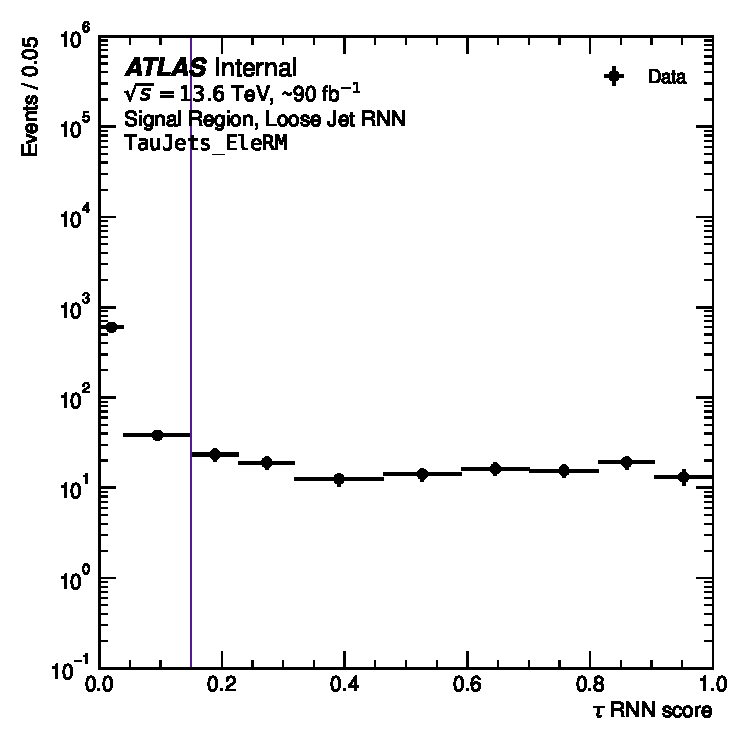
\includegraphics[width=0.50\textwidth]{plotsZtt/erm/erm_best_tau_rnn_SR}
                \label{fig:SR_rnn}
            }
            \subfloat[]{
                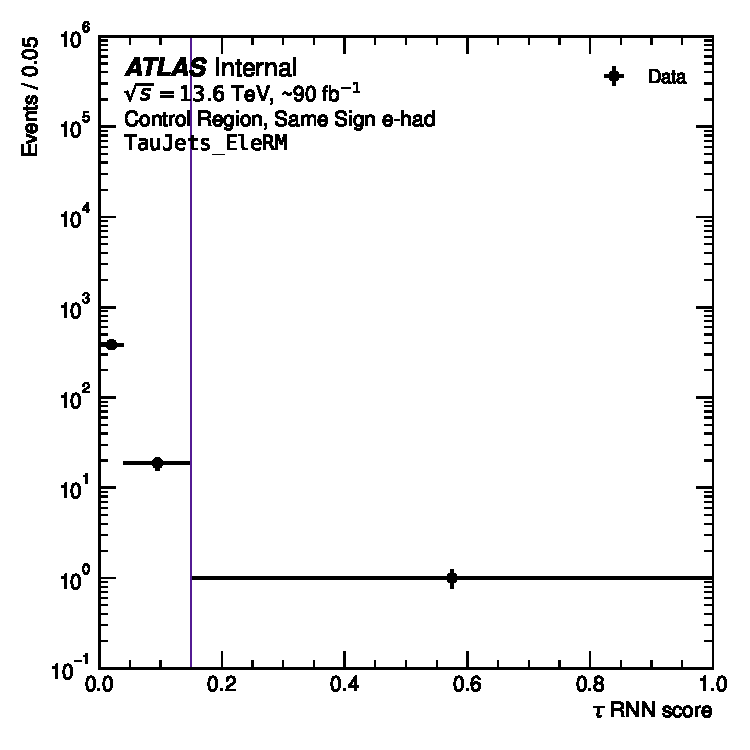
\includegraphics[width=0.50\textwidth]{plotsZtt/erm/erm_best_tau_rnn_CR_SS}
                \label{fig:CR_rnn}
            }
            \caption{
                The distribution of the TauID RNN score: (\protect\subref{fig:SR_rnn}) in the SR, and,
                (\protect\subref{fig:CR_rnn}) in the CR. 
                All requirement criteria are applied, 
                except the requirement on the variable being plotted.
                The vertical line indicates the event-selection requirement on this variable.
            }
            \label{fig:erm:rnn}
        \end{figure}
        \begin{figure}[!tb]
            \centering
            \subfloat[]{
                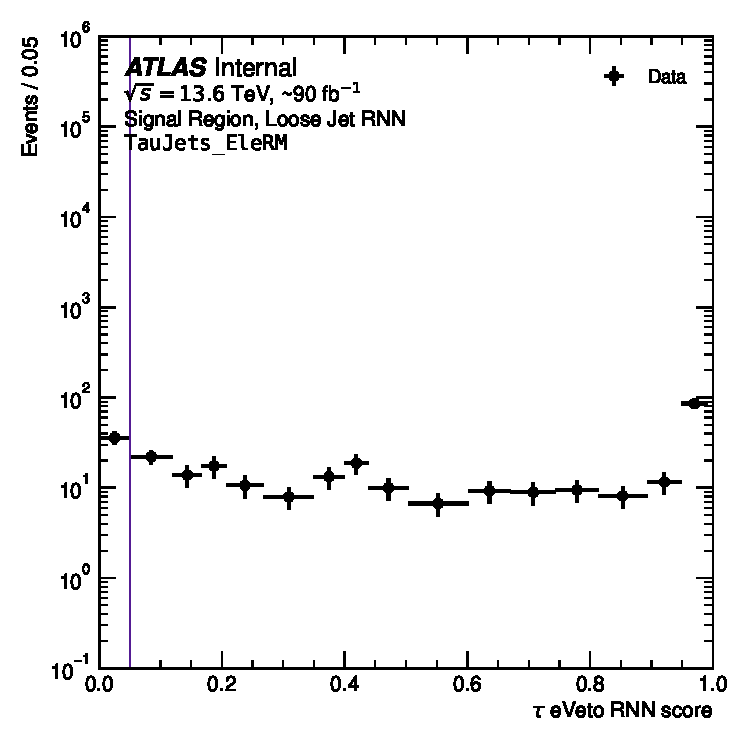
\includegraphics[width=0.50\textwidth]{plotsZtt/erm/erm_best_tau_eveto_rnn_SR}
                \label{fig:SR_eveto_rnn}
            }
            \subfloat[]{
                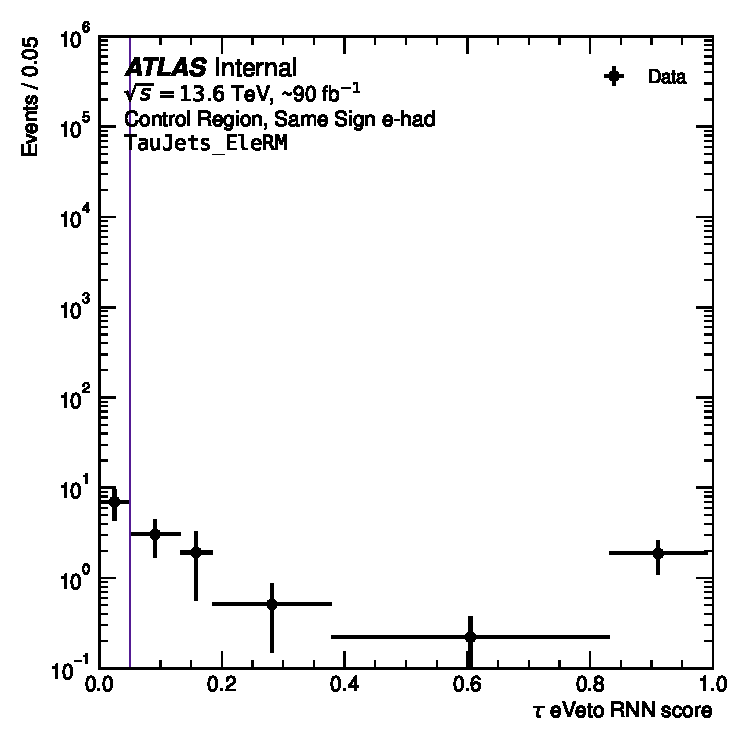
\includegraphics[width=0.50\textwidth]{plotsZtt/erm/erm_best_tau_eveto_rnn_CR_SS}
                \label{fig:CR_eveto_rnn}
            }
            \caption{
                The distribution of the TauID e-veto RNN score: (\protect\subref{fig:SR_eveto_rnn}) in the SR, and,
                (\protect\subref{fig:CR_eveto_rnn}) in the CR. 
                All requirement criteria are applied, 
                except the requirement on the variable being plotted.
                The vertical line indicates the event-selection requirement on this variable.
            }
            \label{fig:erm:eveto_rnn}
        \end{figure}
        
        It is encouraging to see that the distribution of \mcolEtau has the same shape 
        as the \mcol in the \Zttmuhad channel, featuring a peak at the Z boson mass and 
        a shoulder in the low-mass region. The shape of the \mcolEtau distribution for signal 
        Drell-Yan events seen in Figure~\ref{fig:erm:m_col} is very different from that seen
        in inclusive production, with a much larger fraction of the signal events in the 
        region $40 < \mcolEtau < 70$ GeV relative to that at the Z boson peak.  
        This is a result of the sharply falling distribution in Z boson \pT for Drell-Yan 
        production, coupled with the fact that the opening angle of boosted \teth systems 
        decreases with decreasing \mcolEtau.
        The \ptcolEtau distribution in the SR shows 
        a peak at a transverse momentum of around 450~\GeV, also consistent with the 
        \ptcol distribution in the \Zttmuhad channel. 
        The jet RNN distribution in the SR is statistically consistent with a flat distribution,
        in the higher RNN score region, indicating a high signal purity in the SR.
        An increase in the event yield at the low 
        RNN score region is observed in the SR, indicating a non-negligible 
        background contribution. This is in line with the CR jet RNN distribution.
        The electron-veto RNN distribution shows a bump in the low-score region, 
        indicating a non-negligible contribution from electron background.

        Figure~\ref{fig:erm:SRcmp} shows comparisons between the event yield for 
        \mcolEtau\ distributions corresponding to various SR definitions,
        each mirroring the \tauhadmurm benchmark. 
        Figure~\ref{fig:erm:SR_m} shows the nominal SR. 
        Figure~\ref{fig:erm:SR_std_m} shows the sample \SRstd. 
        Figure~\ref{fig:SR_tight_m} shows the sample \SRtight.
        Figure~\ref{fig:SR_tight_std_m} shows the sample \SRtightstd.
        \begin{figure}[!tb]
            \centering
            \subfloat[]{
                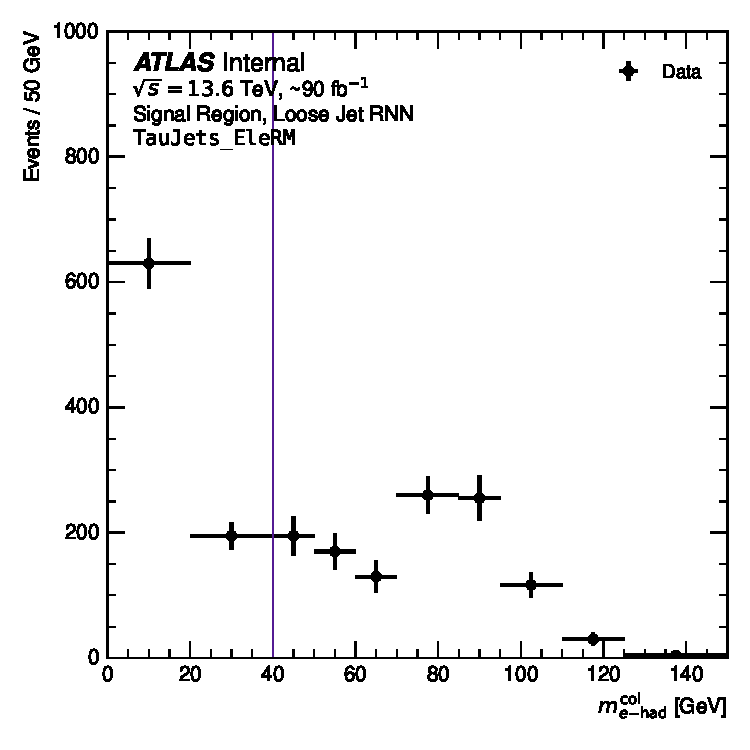
\includegraphics[width=0.50\textwidth]{plotsZtt/erm/erm_m_tt_colin_SR}
                \label{fig:erm:SR_m}
            }
            \subfloat[]{
                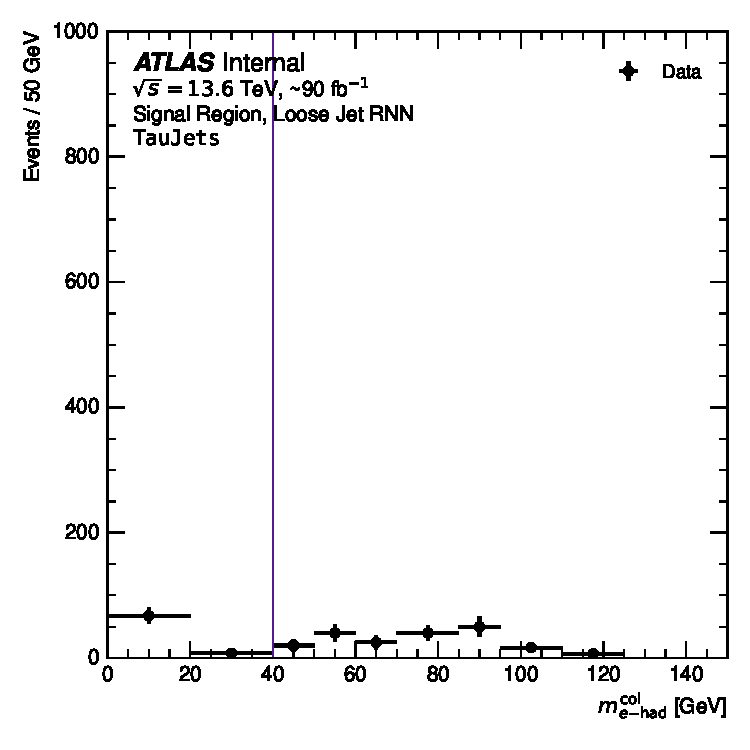
\includegraphics[width=0.50\textwidth]{plotsZtt/std/std_m_tt_colin_SR}
                \label{fig:erm:SR_std_m}
            }
            \\
            \subfloat[]{
                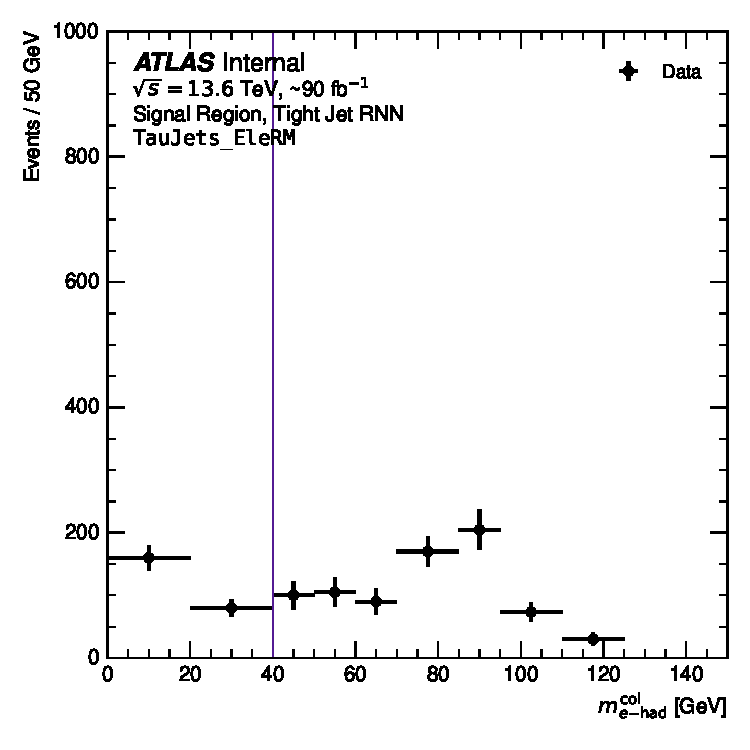
\includegraphics[width=0.50\textwidth]{plotsZtt/erm/erm_m_tt_colin_SR_tight}
                \label{fig:SR_tight_m}
            }
            \subfloat[]{
                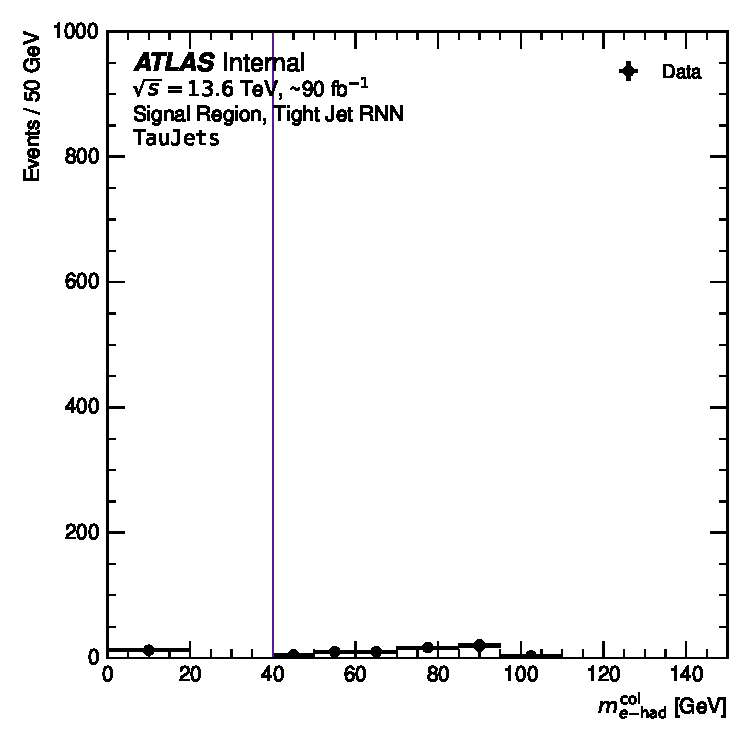
\includegraphics[width=0.50\textwidth]{plotsZtt/std/std_m_tt_colin_SR_tight}
                \label{fig:SR_tight_std_m}
            }
            \caption{
                The distribution of the $\mcolEtau$ in the SR: (\protect\subref{fig:erm:SR_m}) nominal SR, 
                (\protect\subref{fig:erm:SR_std_m}) \SRstd, 
                (\protect\subref{fig:SR_tight_m}) \SRtight, and,
                (\protect\subref{fig:SR_tight_std_m}) \SRtightstd. 
                SR, $\SRtight$ and CR are with the $\tauhaderm$ method, while $\SRstd$ and $\SRtightstd$ are with the standard ATLAS TauID.
            }
            \label{fig:erm:SRcmp}
        \end{figure}

        
        \begin{table}[htbp]
            \caption{
                Event yields in SR and CR. 
                SR, \SRtight, \SRstd, and \SRtightstd are defined mirroring the \tauhadmurm benchmark.
                CR, \CRtight, \CRstd, and \CRtightstd are defined by requiring the same 
                charge electron-$\tauhad$ in the SR, \SRtight, \SRstd, and \SRtightstd, respectively.
                SR, $\SRtight$ and CR are with the $\tauhaderm$ method, while $\SRstd$ and $\SRtightstd$ are with the standard ATLAS TauID.
                The uncertainties quoted are statistical only.
            }
            \label{tab:erm:yield}
            \centering
            % \scriptsize
            \begin{tabular}{l|cc|cc}
                \toprule
                                        & SR           & \SRtight      & \SRstd     & \SRtightstd   \\ 
                \midrule
                Data                    & $274 \pm 17$ & $182 \pm 13$  & $46 \pm 7$ & $15 \pm 4$    \\ 
                \bottomrule
                \toprule
                                        & CR           & \CRtight      & \CRstd     & \CRtightstd   \\ 
                \midrule
                Data                    & $15 \pm 4$   & $5 \pm 2$     & $3 \pm 2$  & $1 \pm 1$     \\
                \bottomrule
            \end{tabular}
        \end{table}
        The event yields in the various SR and CR are shown in Table \ref{tab:erm:yield}. 
        Without MC samples, the signal and background levels in the SR can only be estimated 
        using the TauID efficiency and the event yields in the CR. To estimate the signal 
        and background levels in the SR, we make the following assumptions:
        \begin{itemize}
            \item The TauID efficiency in the SR is the same as the TauID efficiency observed when flattening the RNN score.
            \item The increase in TauID background rejection power when moving from the Loose to Tight WP is the same in both the SR and CR.
            \item The \Zttehad signal contribution is negligible in the CR.
        \end{itemize}"

        Based on these assumptions, the signal and background levels in the SR can be 
        estimated using the following equations:
        \begin{equation}\begin{split}
            n^\mathrm{SR}_\mathrm{data} &= 85\% \times n^\mathrm{all}_\mathrm{sig} + n^\mathrm{SR}_\mathrm{bkg}, \\
            n^\mathrm{SRtight}_\mathrm{data} &= 60\% \times n^\mathrm{all}_\mathrm{sig} + n^\mathrm{SRtight}_\mathrm{bkg}, \\
        \end{split}\end{equation}
        where:
        \begin{itemize}
            \item \( n^\mathrm{SR}_\mathrm{data} \) is the number of data events in the SR,
            \item \( n^\mathrm{SRtight}_\mathrm{data} \) is the number of data events in the \SRtight,
            \item \( n^\mathrm{all}_\mathrm{sig} \) is the estimated total number of signal events in the SR, before the application of the selection requirement on tau RNN score.
            \item \( n^\mathrm{SR}_\mathrm{bkg} \) is the estimated number of background events in the SR,
            \item \( n^\mathrm{SRtight}_\mathrm{bkg} \) is the estimated number of background events in the \SRtight.
        \end{itemize}
        The ratio of background events between the SR and \SRtight can be estimated from the ratio of data events in the CR and \CRtight:
        \begin{equation}
            \frac{n^\mathrm{SRtight}_\mathrm{bkg}}{n^\mathrm{SR}_\mathrm{bkg}} = \frac{n^\mathrm{CRtight}_\mathrm{data}}{n^\mathrm{CR}_\mathrm{data}},
        \end{equation}
        where:
        \begin{itemize}
            \item \( n^\mathrm{CR}_\mathrm{data} \) is the number of data events in the CR,
            \item \( n^\mathrm{CRtight}_\mathrm{data} \) is the number of data events in the \CRtight.
        \end{itemize}
        By solving these equations, the estimated number of background events in the SR 
        is \( n^\mathrm{SR}_\mathrm{bkg} = 31^{+57}_{-31} \), and the estimated number 
        of signal events in the SR is \( n^\mathrm{SR}_\mathrm{sig} = 243^{+31}_{-57} \). 
        Similarly, the estimated number of signal events in the \SRtight is 
        \( n^\mathrm{SRtight}_\mathrm{sig} = 172^{+10}_{-19} \), and the estimated number 
        of background events in the \SRtight is \( n^\mathrm{SRtight}_\mathrm{bkg} = 10^{+19}_{-10} \).
        Repeating the same process for the \SRstd and \SRtightstd regions yields signal 
        estimations of zero events in both regions, indicating that the assumptions above 
        may not hold in \SRstd and \SRtightstd, or that these regions are background-dominated.
        The estimated signal purity in the SR is \( 88\%^{+12\%}_{-20\%} \), 
        and in the \SRtight it is \( 95\%^{+5\%}_{-11\%} \). All quoted uncertainties are statistical only.
        
        The \tauhaderm\ objects show a significant improvement in signal yield compared to the standard 
        \tauhad\ objects; the background-inclusive yield is six times higher in the SR and 12 times 
        higher in the \SRtight. Compared with the \tauhadmurm\ benchmark, the \tauhaderm\ benchmark 
        exhibits a similar level of signal purity but a lower signal yield. Normalising to unit 
        luminosity, the \tauhadmurm\ benchmark yields $6.8 \pm 0.8$~(syst. + stat.) events per \ifb\ in the SR, 
        while the \tauhaderm\ benchmark yields $2.7^{+0.3}_{-0.6}$ events per \ifb\ in the SR. 
        This corresponds to $40\%^{+6\%}_{-10\%}$ of the \tauhadmurm\ benchmark yield.

        The difference in signal yield is entirely expected. The \tauhaderm\ algorithm has a lower 
        reconstruction and identification efficiency (roughly 70\% of that of the \tauhadmurm\ objects); 
        the trigger efficiency is lower (less than 80\% of the \tauhadmurm\ benchmark); 
        the TauID requirements are tighter (90\% of the \tauhadmurm\ benchmark); 
        The Z boson production cross-section increases by 5\% 
        with the centre of mass energy change from 13~\TeV to 13.6~\TeV\ 
        is expected~(105\%).
        Combining these factors, the expected SR signal yield should be around 53\%
        of the \tauhadmurm\ benchmark, 
        which is higher than the observed $40\%^{+6\%}_{-10\%}$.
        The difference can be attributed to the systematic uncertainties in the
        TauID efficiency, the trigger efficiency, and the Z boson production cross-section.

\section{Summary and outlook}
    \label{sec:erm:summary}
    In this chapter, we have considered the case of a highly boosted pair 
    of $\tau$ leptons, where one $\tau$ decays to produce an electron and 
    the other $\tau$ decays hadronically. In such cases, the visible decay 
    products are reconstructed within a single $\tauseed$ jet.

    We have described the development of an electron-removal procedure 
    using samples of high-mass $\GHHFourtau$ events. We have demonstrated 
    that this $\tauhaderm$ method recovers the \tauhad\ identification 
    efficiency back to the level expected for isolated \tauhad\ decays 
    for all TauID working points when the electron is properly removed. 
    The measurement precision for the kinematic properties of the 
    visible \tauhad\ system is similarly recovered. We have benchmarked 
    the $\tauhaderm$ objects by selecting a sample of highly boosted 
    $\Zttehad$ final states using the partial 90~\ifb\ Run 3 dataset 
    recorded by the ATLAS detector in 2024 at a centre-of-mass energy of 13.6~\TeV.

    We found that the $\tauhaderm$ objects have a significant improvement 
    in the \teth\ reconstruction efficiency, with an event yield of 
    $274 \pm 17$ in the SR --- six times higher than the standard \tauhad\ 
    objects, and 12 times higher if the \SRtight\ is considered. 
    The signal purity in the SR is estimated to be $88\%^{+12\%}_{-20\%}$, 
    and in the \SRtight\ it is estimated to be $95\%^{+5\%}_{-11\%}$, 
    comparable to the \tauhadmurm\ benchmark. The limited event yields 
    in the CR highlight the success in suppressing background contributions.

    This study, together with the \tauhadmurm\ benchmark, demonstrates 
    that the lepton-removal \tauhad\ reconstruction is ready for physics 
    analysis at the ATLAS experiment. These lepton-removal objects lay the 
    foundation for future searches for high-mass BSM resonances in the 
    $\tau_\text{lep}\tau_\text{had}$ channel. They also open up exciting 
    opportunities for exploring other new physics phenomena at the 
    ATLAS experiment. 